%\subsection{2. Fundamentos de la mecánica de fluidos}
\begin{frame}{Ejercicio}
\justifying
Considerando un fluido unidimensional en densidad y viscosidad para un flujo en una tubería con una presión de entrada pi, y una presión de salida po con un randio del tubo r y una longitud l, la densidad del fluido puede ser representado como p. Expresado el esfuerzo cortante de la pared como una función de las variables. \\
{\tiny Tomado del libro engineering por David Rubestein, pagina 58, problema 2.7 .}
\end{frame}

%*******************************************
%\subsection{1. Cinemática}
\begin{frame}{Cinemática 01/02}
\justifying
La cinemática es el estudio de movimiento de los fluidos sin la necesidad de considerar la naturaleza de las fuerzas o momentos que la originen. Esto implica estudiar la velocidad.
Existen dos métodos para estudiar la cinmática de los fluidos.
\begin{itemize}
\item El método Lagrangiano
\item El método Euleriano (más realístico).
\end{itemize}
{\tiny Tomado del libro Biofluid Mechanics Principles Ali Ostadfar, pagina 10.}
\end{frame}
	
\begin{frame}{Cinemática 02/02}
\justifying
\begin{figure}[H]
\centering
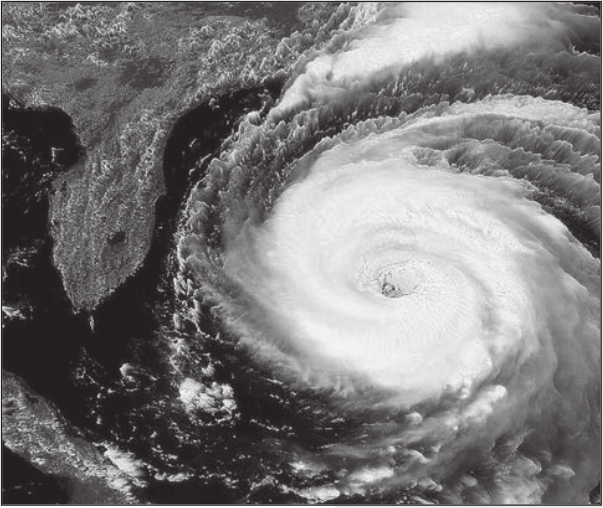
\includegraphics[scale=0.2]{Section_Files/imagenes/sec02_0400_Fig02-00.png}
\caption{Imagen satelital de un huracán cerca de la costa de Florida. Las pequeñas gotas de agua se mueven con el aire, lo cual permite visualizar el movimiento en remolino en sentido contrario al de las manecillas del reloj.}
\label{fig: Figura2-Fig02-00}
\end{figure}
{\tiny Tomada de Fundamentos y Aplicaciones de Mecánica de Fluidos de Yunus Cengel y John Cimbala.}
\end{frame}

%*******************************************

\begin{frame}{Método Lagrangiano}
\justifying
\begin{itemize}
\item Más apropiado para mecánica de sólidos.
\item Analiza al cuerpo como una partícula.
\item Estudia la posición del cuerpo en función al tiempo.
\end{itemize}
\begin{figure}
\centering
\subfloat[Volúmen de control]{
\label{f:imagen1}
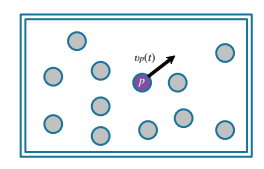
\includegraphics[height=0.15\textwidth]{Section_Files/picmanuel/01.png}}
\subfloat[Sistema de referencia]{
\label{f:imagen2}
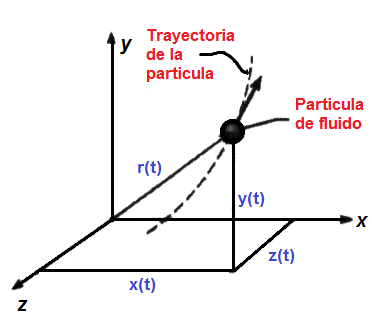
\includegraphics[height=0.15\textwidth]{Section_Files/picmanuel/02.png}}
\caption{Caso lagrangiano}
\label{f:casolagrangiano}
\end{figure}			
{\tiny Tomada del libro Biofluid Mechanics Principles, Ali Ostadfar, página 10.}
\end{frame}	

\begin{frame}{Método Euleriano 01/03}
\justifying
\begin{itemize}
\item Más apropiado para mecánica de fluidos.
\item Las propiedades del flui9do son caracterizados en 4 dimensiones (x,y,z y t).
\item El campo de velocidad v(x,y,z,t) o presión p(x,y,z,t) no es igual a v(t) o p(t).
\item Analiza al cuerpo como un volumen de control.
\item Estudia al campo de velocidades.
\end{itemize}
\begin{figure}[H]
\centering
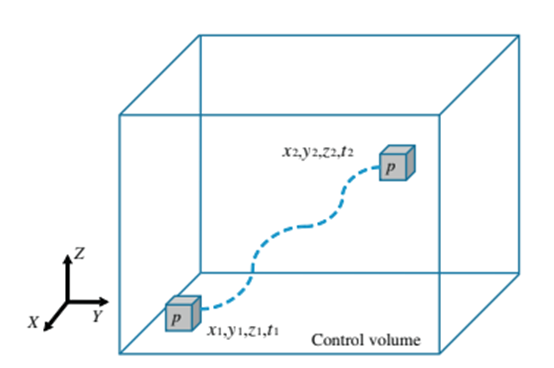
\includegraphics[scale=0.2]{Section_Files/picmanuel/03.png}
\caption{El volumen de control (V.C.) es un volumen finito por el cual el fluido entra o sale. El V.C. puede ser rígido, flexible, estático o en movimiento.}
\label{fig: Figura2-Fig0403-00}
\end{figure}
{\tiny Tomada del libro Biofluid Mechanics Principles, Ali Ostadfar, página 11.}
\end{frame}

\begin{frame}{Método Euleriano 02/03}
\justifying
Campo de velocidades:
\begin{figure}[H]
\centering
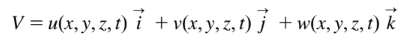
\includegraphics[scale=0.4]{Section_Files/picmanuel/04.png}
\label{fig: Figura2-Fig0403-01}
\end{figure}
Campo de aceleraciones:
\begin{figure}[H]
\centering
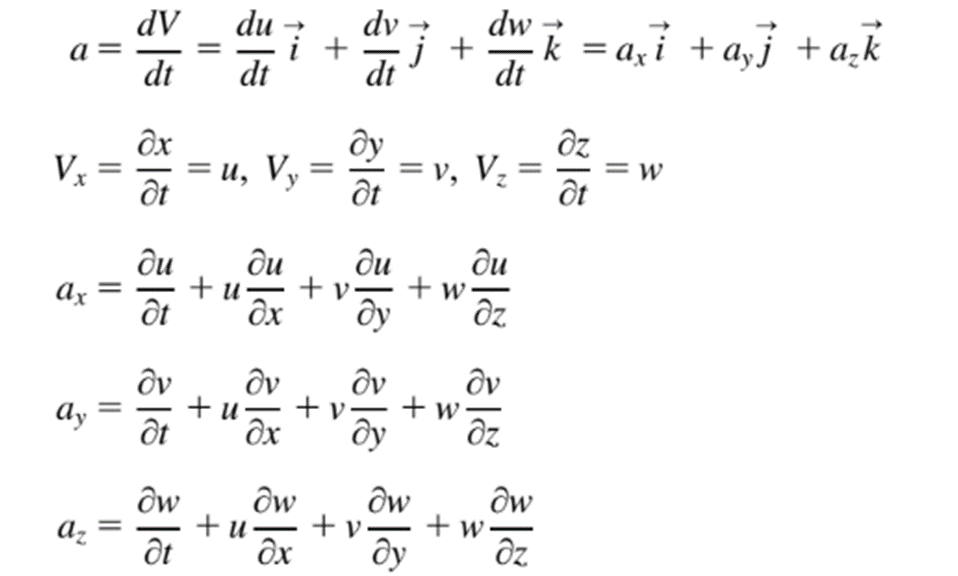
\includegraphics[scale=0.3]{Section_Files/picmanuel/05.png}
\label{fig: Figura2-Fig0403-02}
\end{figure}
{\tiny Tomada del libro Biofluid Mechanics Principles, Ali Ostadfar, página 12.}
\end{frame}	

\begin{frame}{Método Euleriano 03/03}
\justifying
Aceleración convectiva:
\begin{figure}[H]
\centering
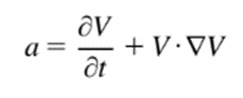
\includegraphics[scale=0.4]{Section_Files/picmanuel/06.png}
%\caption{El volumen de control (V.C.) es un volumen finito por el cual el fluido entra o sale. El V.C. puede ser rígido, flexible, estático o en movimiento.}
\label{fig: Figura2-Fig0403-03}
\end{figure}
Líneas de flujo: Este método es una de las mejores herramientas para estudiar un campo de fluidos.
\begin{itemize}
\item Líneas de corriente.
\item Líneas de trayectoria.
\item Líneas de traza.
\item Líneas fluidas.
\end{itemize}
\begin{figure}[H]
\centering
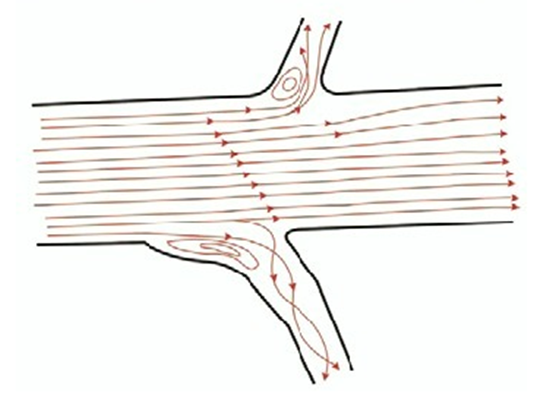
\includegraphics[scale=0.2]{Section_Files/picmanuel/07.png}
%\caption{El volumen de control (V.C.) es un volumen finito por el cual el fluido entra o sale. El V.C. puede ser rígido, flexible, estático o en movimiento.}
\label{fig: Figura2-Fig0403-04}
\end{figure}
{\tiny Tomada del libro Biofluid Mechanics Principles, Ali Ostadfar, página 12.}
\end{frame}	

\begin{frame}{Líneas de corriente}
\justifying
Es una línea curva que, en todas partes, es tangente al vector de velocidad local instantánea.
Las líneas de corriente no se puieden conocer experimentalmente, excepto en condición de flujo estacionario en los cuales coinciden con las líneas de trayectoria y las líneas de traza.
\begin{figure}
\centering
\subfloat[01]{
\label{f:imagen3}
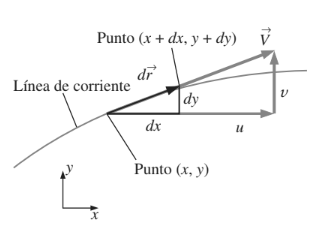
\includegraphics[height=0.25\textwidth]{Section_Files/picmanuel/08.png}}
\subfloat[02]{
\label{f:imagen4}
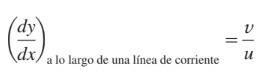
\includegraphics[height=0.10\textwidth]{Section_Files/picmanuel/09.png}}
\caption{La constante de integración es la familia de curvas que satisfacen la ecuación.}
\label{f:casoeuleriano}
\end{figure}	
{\tiny Tomada del libro Biofluid Mechanics Principles, Ali Ostadfar, página 139.}
\end{frame}	

\begin{frame}{Líneas de trayectoria}
\justifying
Una línea de trayectoria es la trayectoria real recorrida por una partícula de fluido durante algún periodo.
Una línea de trayectoria es lo mismo que el conjunto de las ubicaciones de la punta del vector de posición material (xpartícula(t), ypartícula(t), zpartícula(t)) al que se le sigue el rastro durante algún intervalo finito.
\begin{figure}[H]
\centering
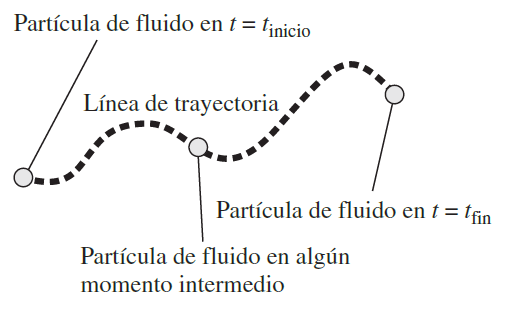
\includegraphics[scale=0.3]{Section_Files/picmanuel/10.png}
\caption{Se forma una línea de trayectoria cuando se sigue la trayectoria real de una partícula de fluido.}
\label{fig: Figura2-Fig0403-05}
\end{figure}	
{\tiny Tomada del libro Biofluid Mechanics Principles, Ali Ostadfar, página 140, 141.}
\end{frame}

\begin{frame}{Líneas de traza}
\justifying
Una línea de traza es el lugar geométrico de las partículas de fluido que han pasado de manera secuencial por un punto prescrito en el flujo.
Si se inserta un tubo pequeño en un flujo y se introduce una corriente continua de fluido trazador (tinte en un flujo de agua o humo en flujo de aire), el patrón que se observa es una línea de traza.
\begin{figure}[H]
\centering
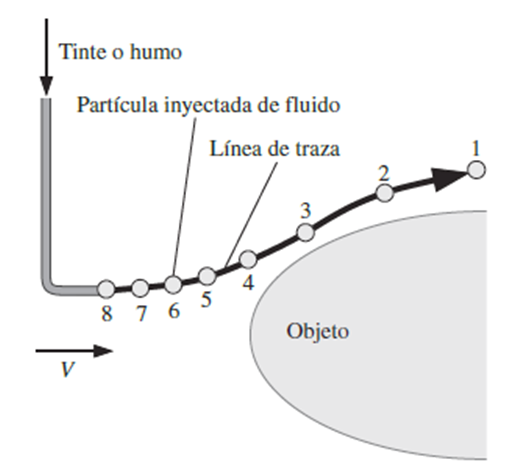
\includegraphics[scale=0.3]{Section_Files/picmanuel/11.png}
\caption{Se forma una línea de traza por la introducción contínua de tinte o humo desde un punto en el flujo. Las partículas trazadoras numeradas (1 a 8) se introdujeron de manera secuencial.}
\label{fig: Figura2-Fig0403-06}
\end{figure}	
{\tiny Tomada del libro Biofluid Mechanics Principles, Ali Ostadfar, página 142.}
\end{frame}

\begin{frame}{Líneas fluidas}
\justifying
Una línea fluida es un conjunto de partículas adyacentes de fluido que se marcaron en el mismo instante (anterior).
Las líneas fluidas son particularmente útiles para situaciones en donde se va a examinar la uniformidad de un flujo (o la falta de ello).
\begin{figure}[H]
\centering
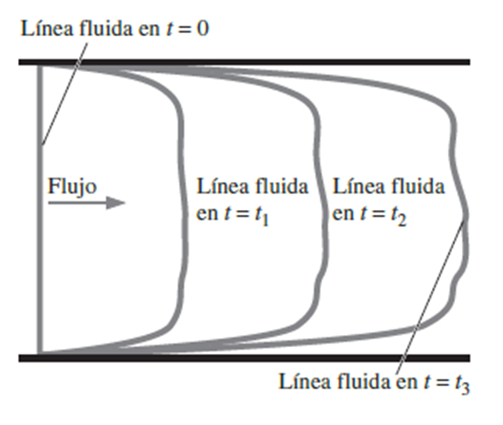
\includegraphics[scale=0.4]{Section_Files/picmanuel/12.png}
\caption{Las líneas fluidas se forman marcando una línea de partículas de fluido y, a continuación, se observa el movimineot (y la deformación) de esa línea a través del campo de flujo; se muestran las líneas fluidas en t0, t1, t2, t3.}
\label{fig: Figura2-Fig0403-07}
\end{figure}	
{\tiny Tomada del libro Biofluid Mechanics Principles, Ali Ostadfar, página 144.}
\end{frame}

\begin{frame}{Ejemplo 01 - 01/02}
\justifying
\begin{figure}[H]
\centering
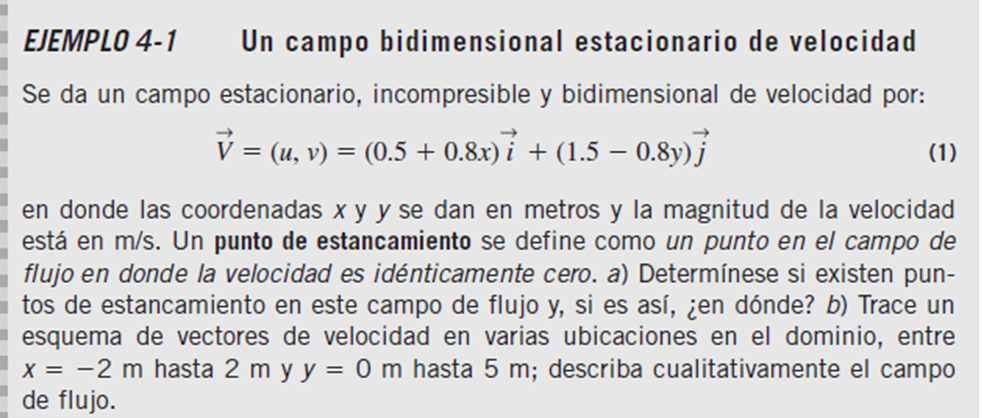
\includegraphics[scale=0.6]{Section_Files/picmanuel/13.png}
\label{fig: Figura2-Fig0403-08}
\end{figure}	
{\tiny Tomada del libro Mecánica de Fluidos por Yunus A. Cengel, página 138.}
\end{frame}

\begin{frame}{Ejemplo 01 - 02/02}
\justifying
\begin{figure}[H]
\centering
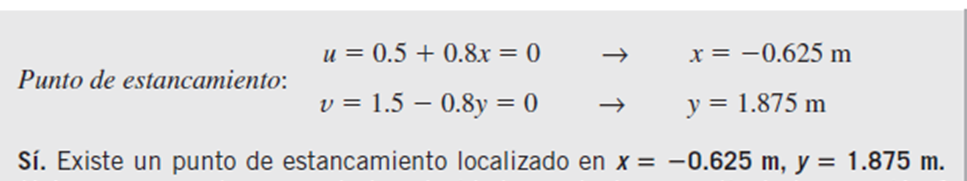
\includegraphics[scale=0.3]{Section_Files/picmanuel/14.png}
\label{fig: Figura2-Fig0403-09}
\end{figure}
\begin{figure}[H]
\centering
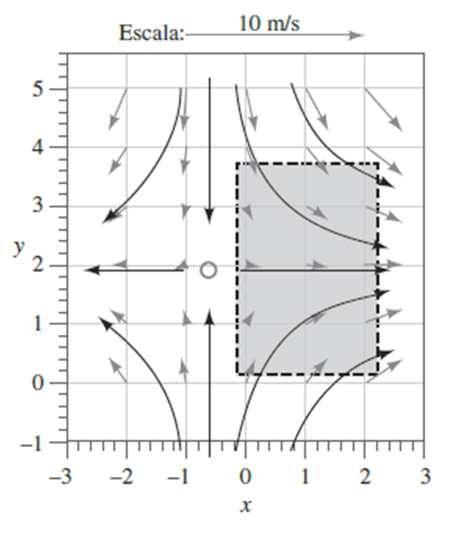
\includegraphics[scale=0.3]{Section_Files/picmanuel/15.png}
\label{fig: Figura2-Fig0403-10}
\end{figure}
{\tiny Tomada del libro Mecánica de Fluidos por Yunus A. Cengel, página 138.}
\end{frame}

\begin{frame}{Ejemplo 02 - 01/03}
\justifying
\begin{figure}[H]
\centering
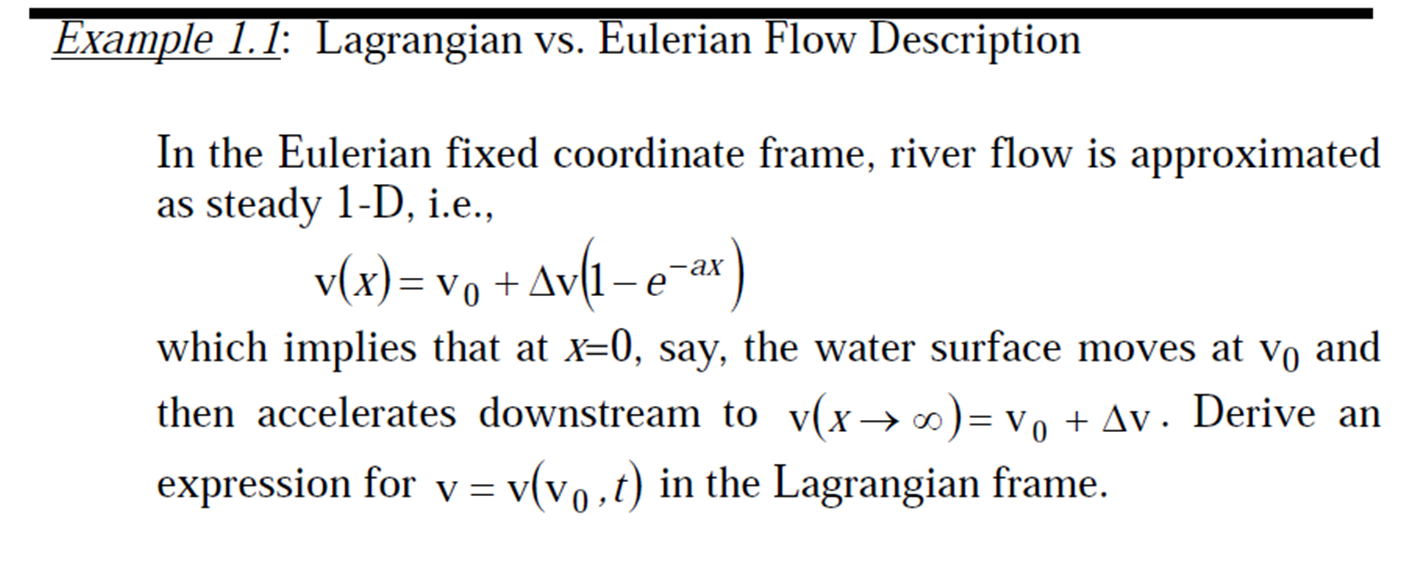
\includegraphics[scale=0.4]{Section_Files/picmanuel/16.png}
\label{fig: Figura2-Fig0403-11}
\end{figure}
{\tiny Tomada del libro Biofluid Dynamics Principles and Select Applications by Celment Kleinstreuer, página 22, 23.}
\end{frame}

\begin{frame}{Ejemplo 02 - 02/03}
\justifying
\begin{figure}[H]
\centering
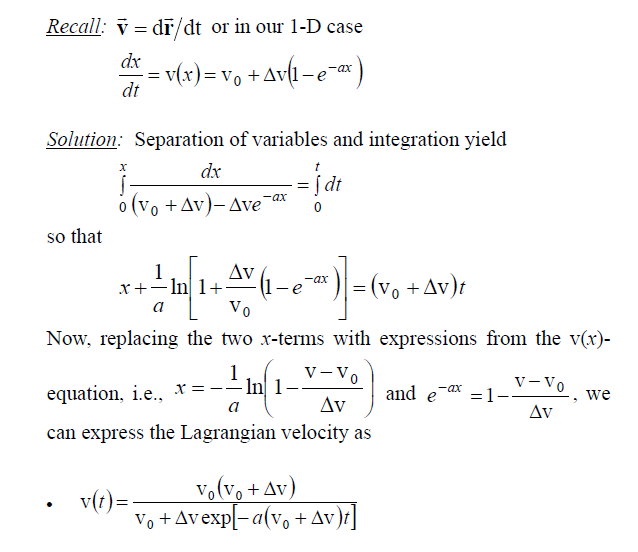
\includegraphics[scale=0.4]{Section_Files/picmanuel/17.png}
\label{fig: Figura2-Fig0403-12}
\end{figure}
{\tiny Tomada del libro Biofluid Dynamics Principles and Select Applications by Celment Kleinstreuer, página 22, 23.}
\end{frame}

\begin{frame}{Ejemplo 02 - 03/03}
\justifying
\begin{figure}[H]
\centering
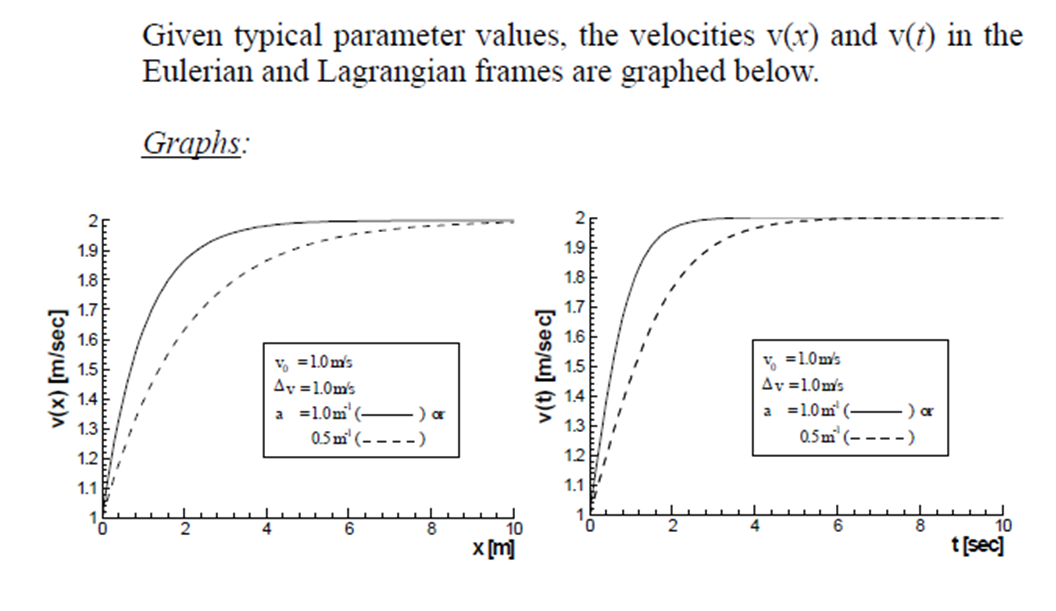
\includegraphics[scale=0.5]{Section_Files/picmanuel/18.png}
\label{fig: Figura2-Fig0403-13}
\end{figure}
{\tiny Tomada del libro Biofluid Dynamics Principles and Select Applications by Celment Kleinstreuer, página 22, 23.}
\end{frame}
%*******************************************


%\subsection{2. Viscosidad}

\begin{frame}{Viscosidad 01/02}
\justifying
Cuando dos cuerpos sólidos en contacto se mueven uno con respecto al otro, se crea una fuerza de fricción en la superficie de contacto en la dirección opuesta al movimiento.
\begin{figure}[H]
\centering
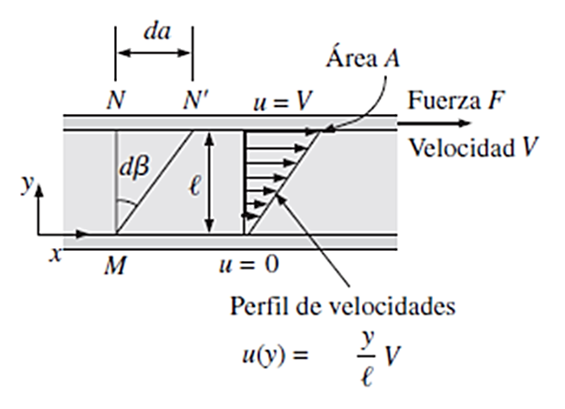
\includegraphics[scale=0.4]{Section_Files/picmanuel/19.png}
\label{fig: Figura2-21}
\end{figure}
{\tiny Tomada del libro Mecánica de Fluidos por Yunus A. Cengel, página 50 y 51.}
\end{frame}

\begin{frame}{Viscosidad 02/02}
\justifying
\begin{figure}
\centering
\subfloat[a.]{
\label{f:imagen6}
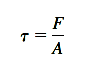
\includegraphics[height=0.10\textwidth]{Section_Files/picmanuel/20.png}}
\subfloat[b.]{
\label{f:imagen7}
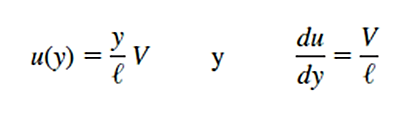
\includegraphics[height=0.10\textwidth]{Section_Files/picmanuel/21.png}}
\subfloat[c.]{
\label{f:imagen8}
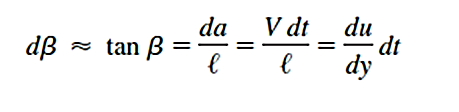
\includegraphics[height=0.08\textwidth]{Section_Files/picmanuel/23.png}}
\caption{Se puede verificar de manera experimental que, para la mayoría de los fluidos, la razón de deformación (y, por lo tanto, el gradiente de velocidad) es directamente proporcional al esfuerzo cortante t.}
\label{f:viscosidad}
\end{figure}
\begin{figure}[H]
\centering
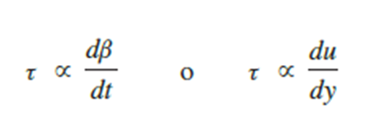
\includegraphics[scale=0.6]{Section_Files/picmanuel/24.png}
\label{fig: Figura2-22}
\end{figure}
{\tiny Tomada del libro Mecánica de Fluidos por Yunus A. Cengel, página 50 y 51.}
\end{frame}

\begin{frame}{Ejemplo 03 - 01/02}
\justifying
\begin{figure}[H]
\centering
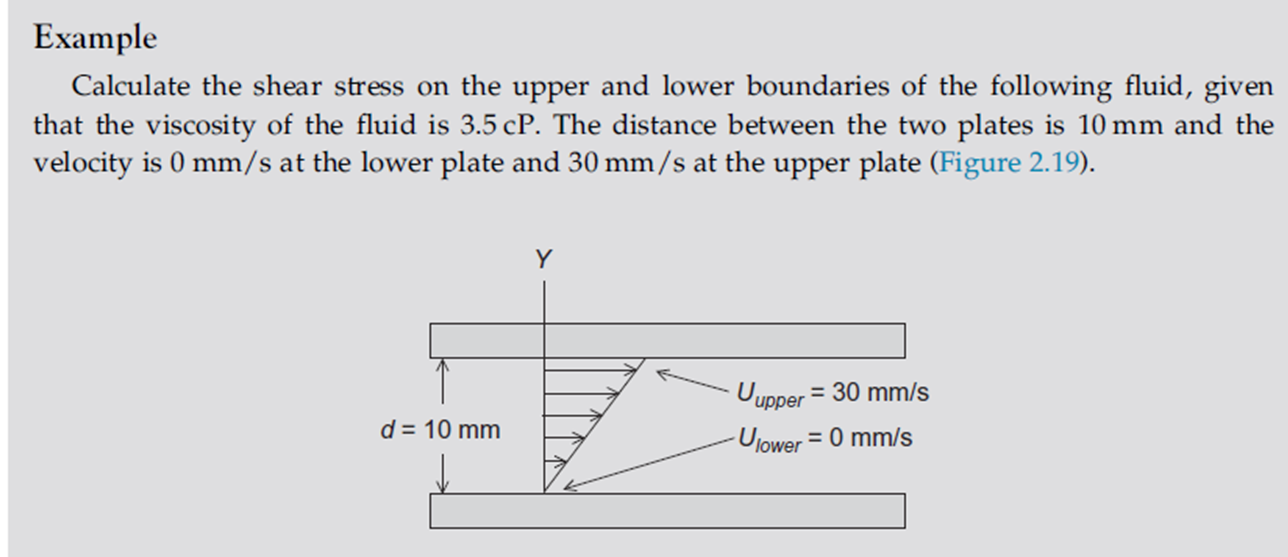
\includegraphics[scale=0.3]{Section_Files/picmanuel/25.png}
\label{fig: Figura2-23}
\end{figure}
{\tiny Tomada del libro Biomedical engineering por David Rubestein, página 43.}
\end{frame}

\begin{frame}{Ejemplo 03 - 02/02}
\justifying
\begin{figure}[H]
\centering
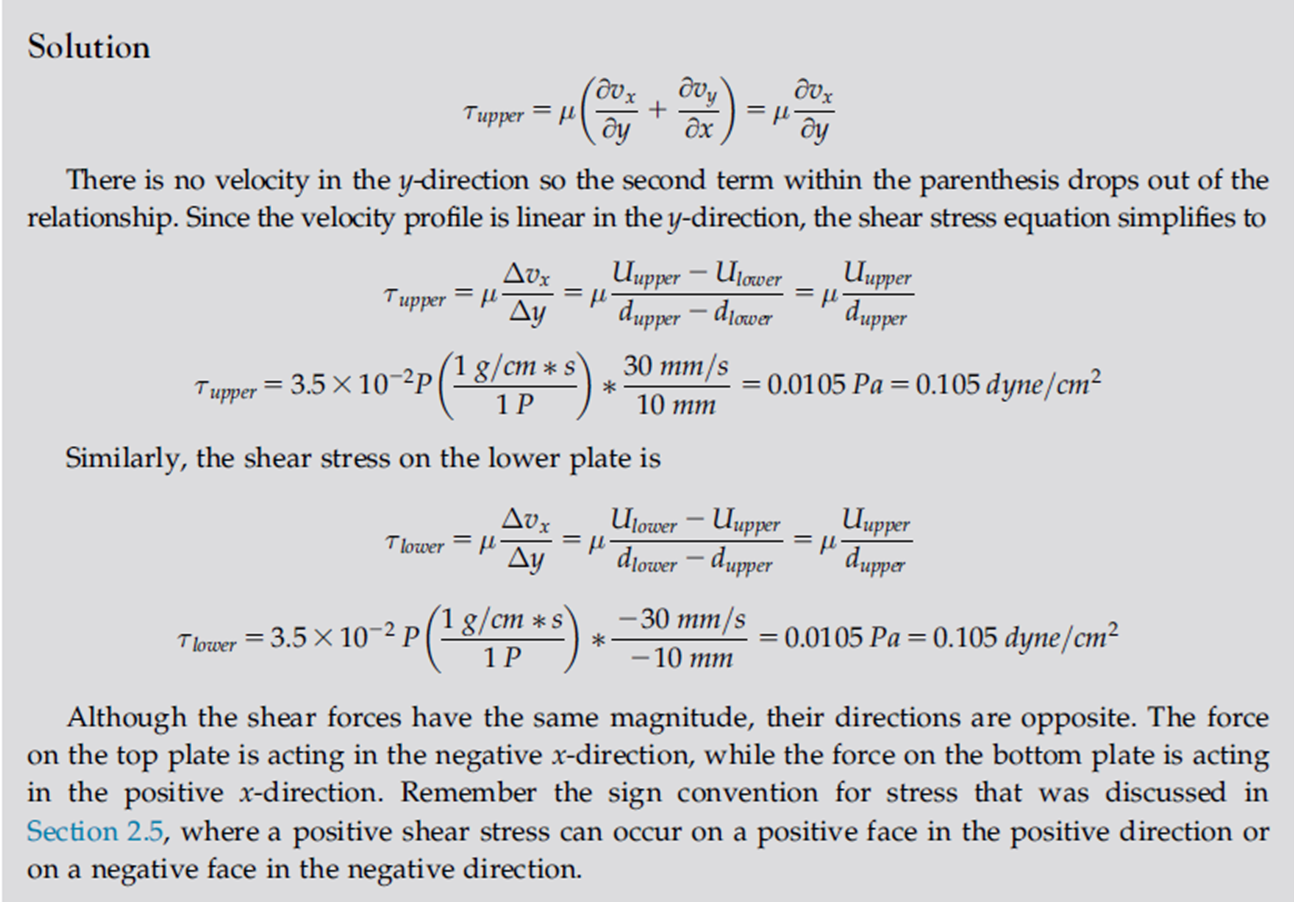
\includegraphics[scale=0.4]{Section_Files/picmanuel/26.png}
\label{fig: Figura2-24}
\end{figure}
{\tiny Tomada del libro Biomedical engineering por David Rubestein, página 43.}
\end{frame}

\begin{frame}{Ejemplo 04}
\justifying
\begin{figure}[H]
\centering
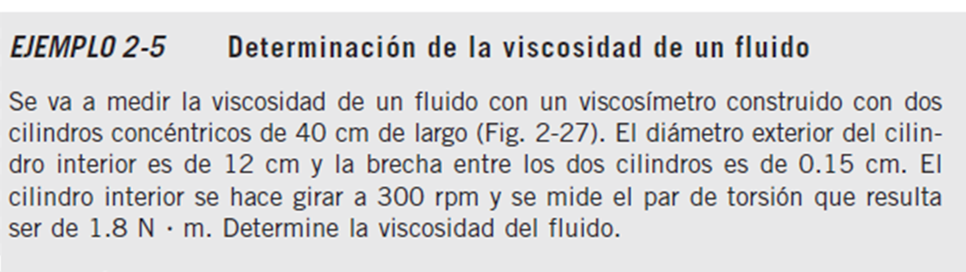
\includegraphics[scale=0.3]{Section_Files/picmanuel/27.png}
\label{fig: Figura2-25}
\end{figure}
\begin{figure}[H]
\centering
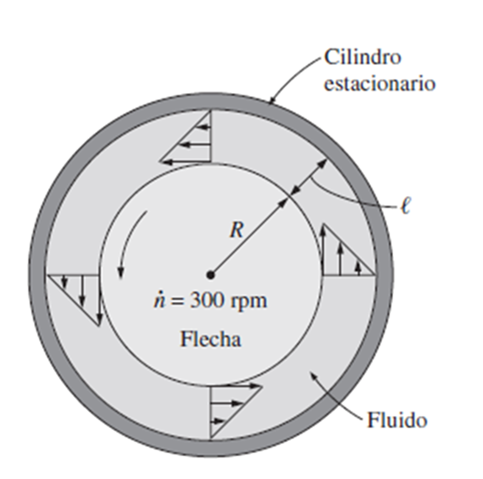
\includegraphics[scale=0.4]{Section_Files/picmanuel/28.png}
\label{fig: Figura2-26}
\end{figure}
{\tiny Tomada del libro Mecánica de Fluidos por Yunus A. Cengel, página 55.}
\end{frame}

\begin{frame}{Ejemplo 05}
\justifying
\begin{figure}[H]
\centering
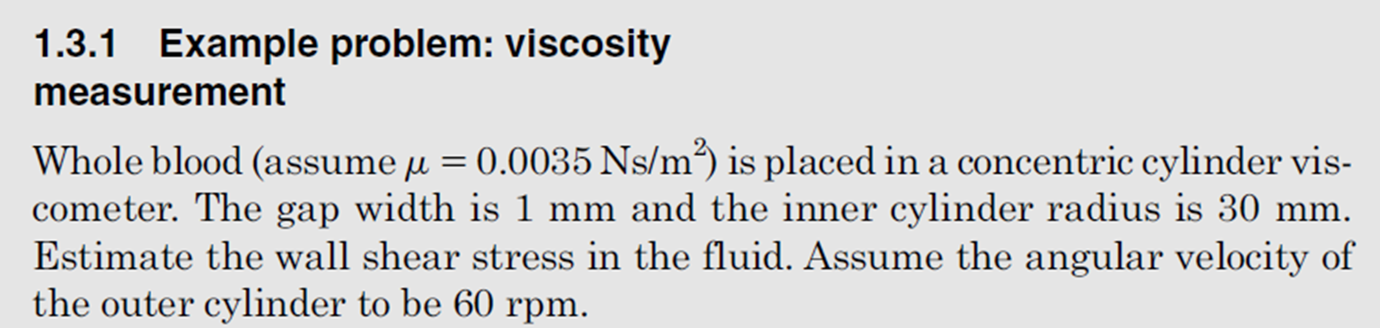
\includegraphics[scale=0.35]{Section_Files/picmanuel/29.png}
\label{fig: Figura2-27}
\end{figure}
\begin{figure}
\centering
\subfloat[a.]{
\label{f:imagen9}
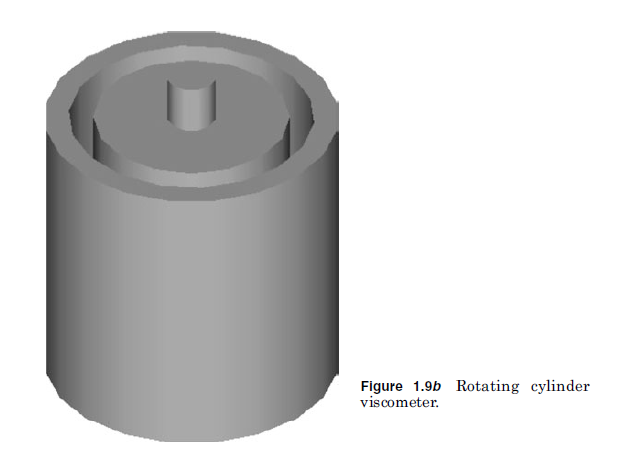
\includegraphics[height=0.20\textwidth]{Section_Files/picmanuel/30.png}}
\subfloat[b.]{
\label{f:imagen10}
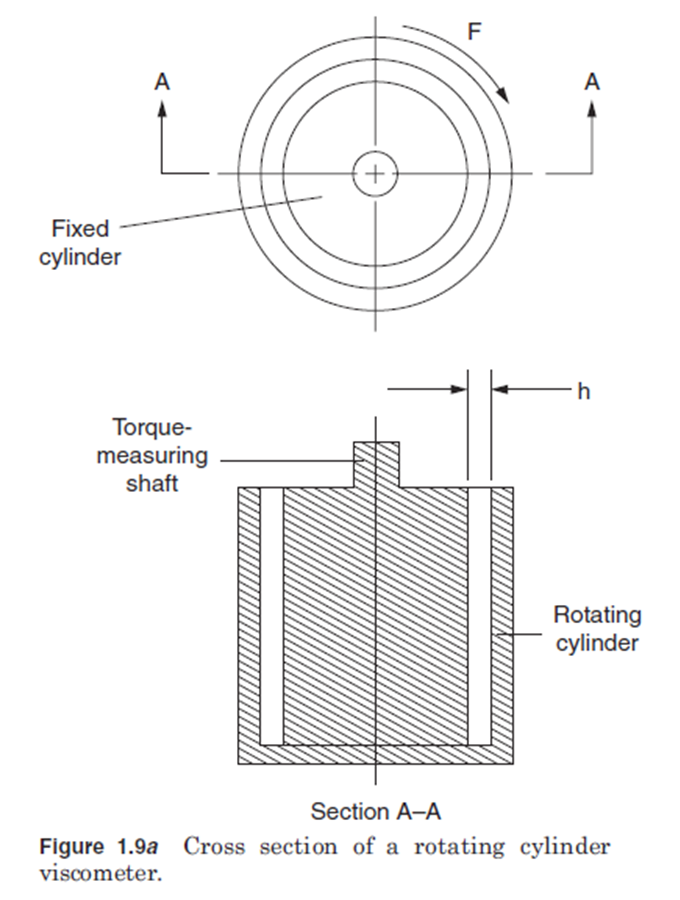
\includegraphics[height=0.20\textwidth]{Section_Files/picmanuel/31.png}}
%\caption{Se puede verificar de manera experimental que, para la mayoría de los fluidos, la razón de deformación (y, por lo tanto, el gradiente de velocidad) es directamente proporcional al esfuerzo cortante t.}
\label{f:ejemplo05}
\end{figure}
{\tiny Tomada del libro Applied Biofluid Mechanics por Lee Wait, página 16.}
\end{frame}
%*******************************************


%\subsection{3. Fluidos Newtoneanos}
\begin{frame}{Fluido Newtoneano y no Newtoneano}
\justifying
Existen tres categorías para los fluidos: fluidos ideales o no viscosos (u=0), fluidos Newtoneanos (u es constante) y los fluidos no Newtoneanos (u varía).
\begin{figure}
\centering
\subfloat[a1.]{
\label{f:imagen11}
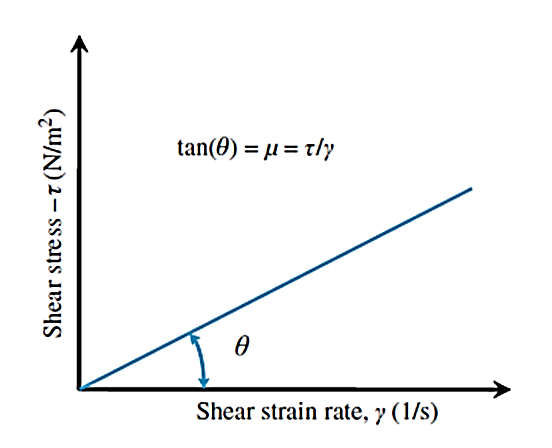
\includegraphics[height=0.30\textwidth]{Section_Files/picmanuel/33.png}}
\subfloat[b2.]{
\label{f:imagen12}
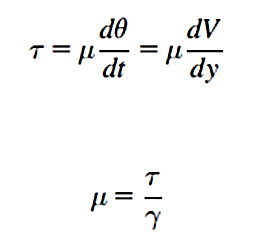
\includegraphics[height=0.30\textwidth]{Section_Files/picmanuel/34.png}}
\caption{Gráfico general de la viscosidad; esfuerzo de corte t vs razón de deformación.}
\label{f:newandnotnew}
\end{figure}
{\tiny Tomada del libro Biofluid Mechanics Principles por Ali Ostadfar, página 15, 16.}
\end{frame}

\begin{frame}{Fluido Newtoneano}
\justifying
\begin{itemize}
\item La viscosidad del aire a 20C es 1.85*10**-5jg/ms y a 60C es 2x10**-5kg/ms.
\item Un incremento en la presión de 1 a 50 atm incrementará la viscosidad del aire en 0.10.
\item Ejemplos de fluido Newtoneano: el agua, el plasma, etc.
\end{itemize}
{\tiny Tomada del libro Biofluid Mechanics Principles por Ali Ostadfar, página 16.}
\end{frame}

\begin{frame}{Fluido No-Newtoneano - 01/02}
\justifying
El coeficiente de viscosidad no es constante, pero esta no es la única condición.
Los fluidos de Boger (u es constante) es un fluido No-Newtoneano, esto debido a que los esfuerzos normales son diferentes de cero.
\begin{figure}[H]
\centering
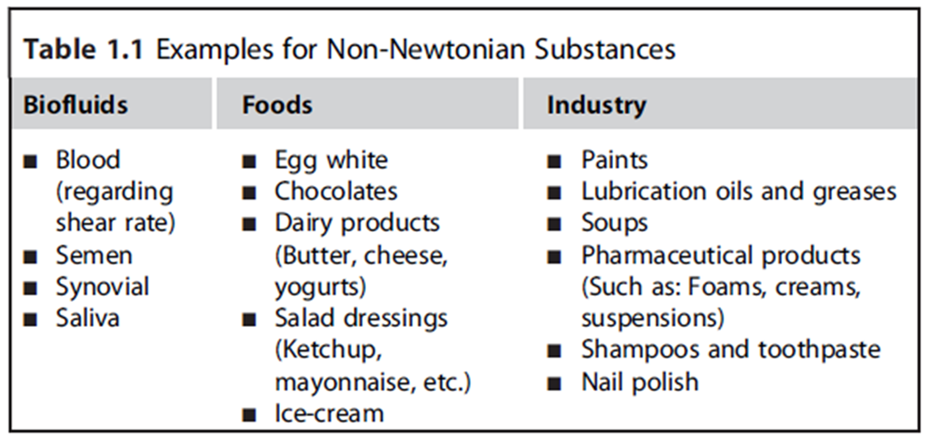
\includegraphics[scale=0.55]{Section_Files/picmanuel/35.png}
\label{fig: Figura2-28}
\end{figure}
{\tiny Tomada del libro Biofluid Mechanics Principles por Ali Ostadfar, página 16.}
\end{frame}

\begin{frame}{Fluido No-Newtoneano - 02/02}
\justifying
Dentro de los fluidos no Newtoneanos existen tres grupos de fluidos:
\begin{itemize}
\item Fluidos independientes del tiempo (dilatantes, seudoplásticos, casson, bingham).
\item Fluidos dependientes del tiempo.
\item Fluidos viscoelásticos.
\end{itemize}
\begin{figure}[H]
\centering
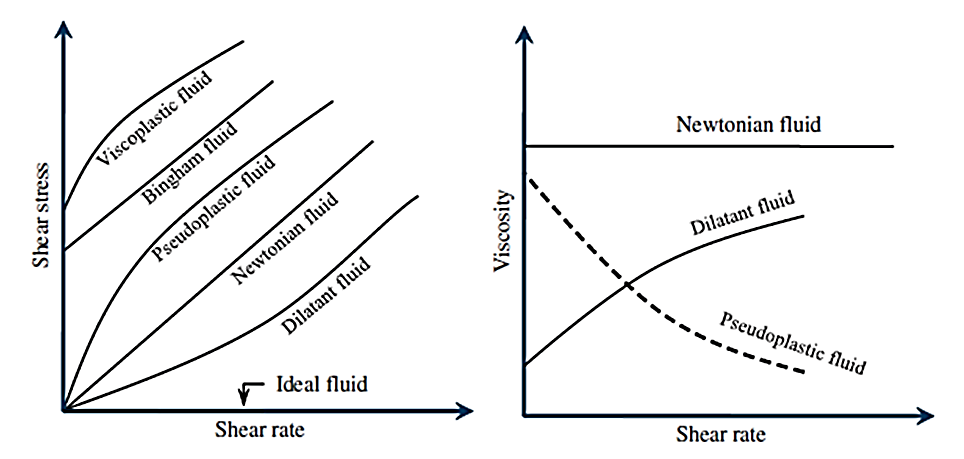
\includegraphics[scale=0.45]{Section_Files/picmanuel/36.png}
\label{fig: Figura2-29}
\caption{Izquierda: Fluidos independientes del tiempo, derecha: Relación de viscosidad vs razón de deformación.}
\end{figure}
{\tiny Tomada del libro Biofluid Mechanics Principles por Ali Ostadfar, página 17.}
\end{frame}

\begin{frame}{Ejemplo 06}
\justifying
\begin{figure}[H]
\centering
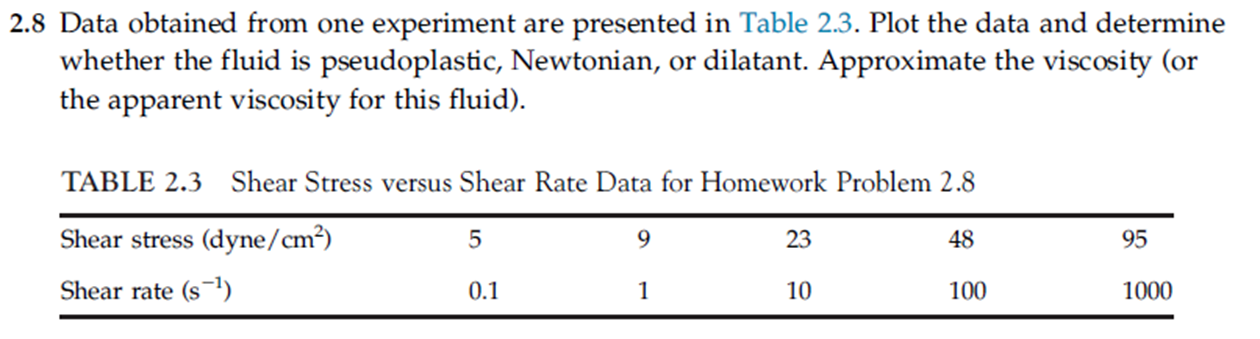
\includegraphics[scale=0.55]{Section_Files/picmanuel/37.png}
\label{fig: Figura2-30}
\end{figure}
{\tiny Tomada del libro Biomedical engineering por David Rubestein, página 58.}
\end{frame}

\begin{frame}{Números adimensionales aplicados a los biofluidos}
\justifying
Los números adimensionales representan una propiedad de un fenómeno físico. Estos números son usados para caracterizar el comportamiento mecánico de un flujo en condición dinámica. En la ingeniería mecánica existen más de 40 números adimensionales, algunos de ellos esenciales para mecánica de biofluidos:
\begin{itemize}
\item Número de Reynolds (Re).
\item Número de Womersely (alpha).
\item Número de Strouhal (St).
\item Número de Dean (De).
\item Número de Stokes (Stk).
\end{itemize}
{\tiny Tomada del libro Biofluid Mechanics Principles por Ali Ostadfar, página 17.}
\end{frame}

\begin{frame}{Números de Reynold (Re) - 01/02}
\justifying
Esta definido como el ratio entre las fuerzas inerciales y las viscosas cuando un fluido fluye a través de una tubería. Este número también sirve para evaluar el régimen de un fluido (laminar o turbulento).
\begin{figure}[H]
\centering
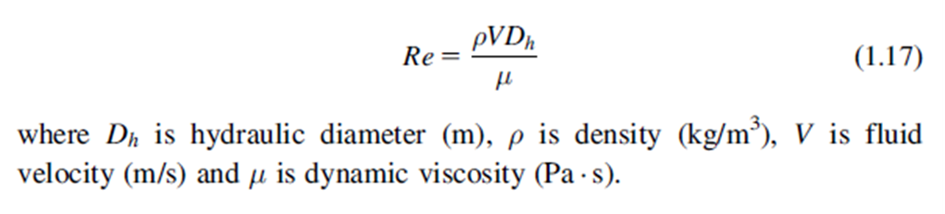
\includegraphics[scale=0.55]{Section_Files/picmanuel/38.png}
\label{fig: Figura2-31}
\end{figure}
{\tiny Tomada del libro Biofluid Mechanics Principles por Ali Ostadfar, página 18.}
\end{frame}

\begin{frame}{Números de Reynold (Re) - 02/02}
\justifying
\begin{figure}[H]
\centering
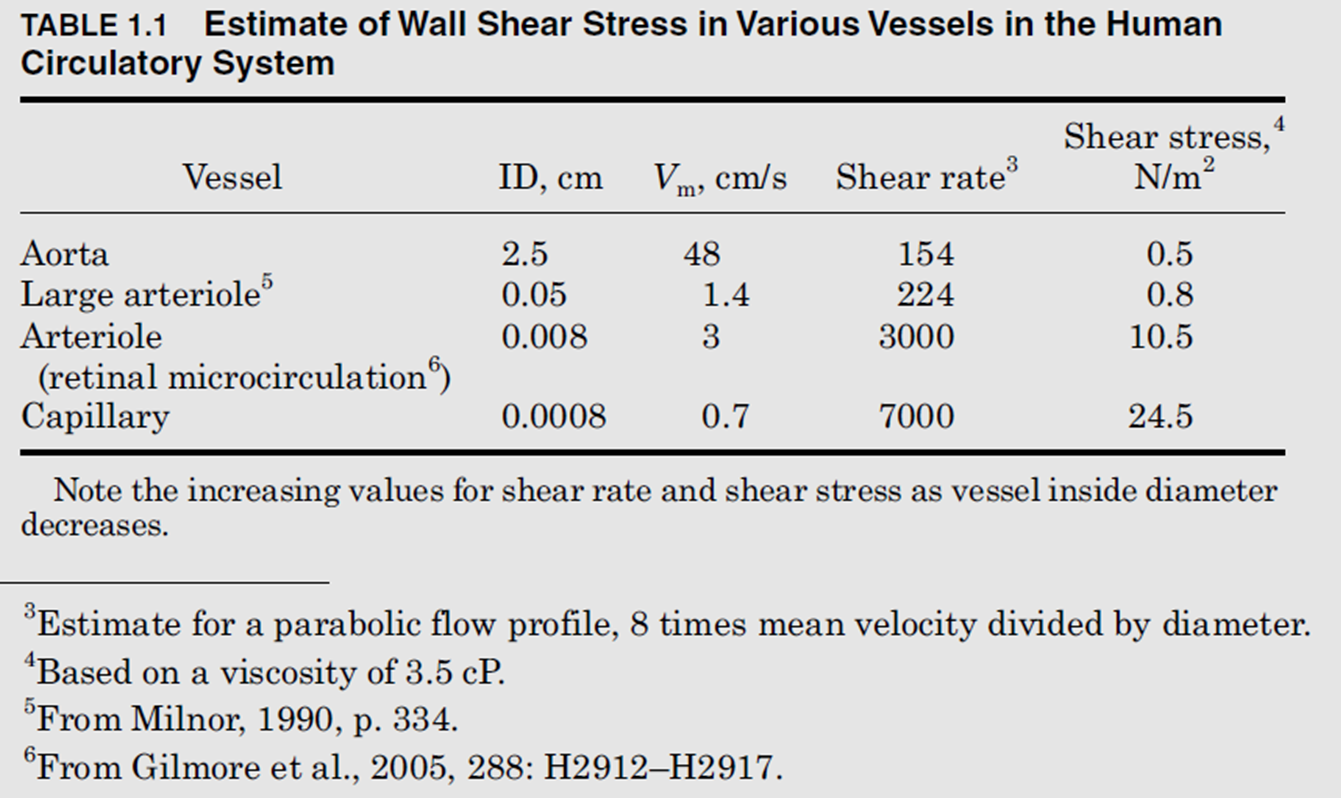
\includegraphics[scale=0.4]{Section_Files/picmanuel/39.png}
\label{fig: Figura2-32}
\end{figure}
{\tiny Tomada del libro Applied Biofluid Mechanics por Lee Wait, página 10.}
\end{frame}

\begin{frame}{Ejemplo 07}
\justifying
\begin{figure}[H]
\centering
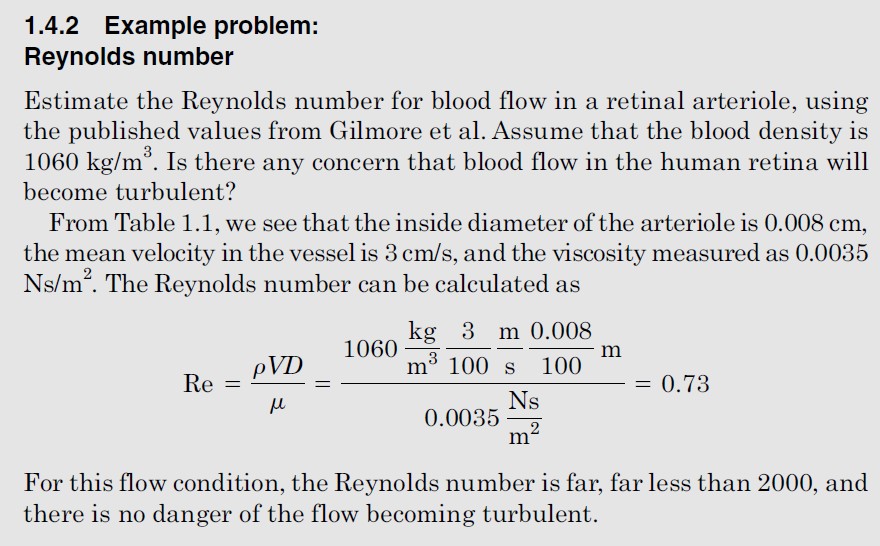
\includegraphics[scale=0.4]{Section_Files/picmanuel/40.png}
\label{fig: Figura2-33}
\end{figure}
{\tiny Tomada del libro Applied Biofluid Mechanics por Lee Wait, página 19.}
\end{frame}

\begin{frame}{Número de Womersely (alpha)}
\justifying
Esta definido como el ratio entre la inercia oscilatoria y los efectos viscosos para un fluido en un flujo pulsátil. El número de Womersley es grande en la aorta y pequeño en las arterioles (menor a 1).
\begin{figure}[H]
\centering
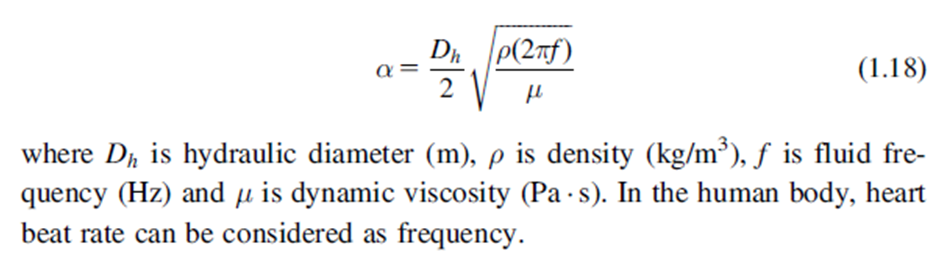
\includegraphics[scale=0.4]{Section_Files/picmanuel/41.png}
\label{fig: Figura2-34}
\end{figure}
{\tiny Tomada del libro Biofluid Mechanics Principles por Ali Ostadfar, página 18.}
\end{frame}

\begin{frame}{Ejemplo 08 - 01/03}
\justifying
\begin{figure}[H]
\centering
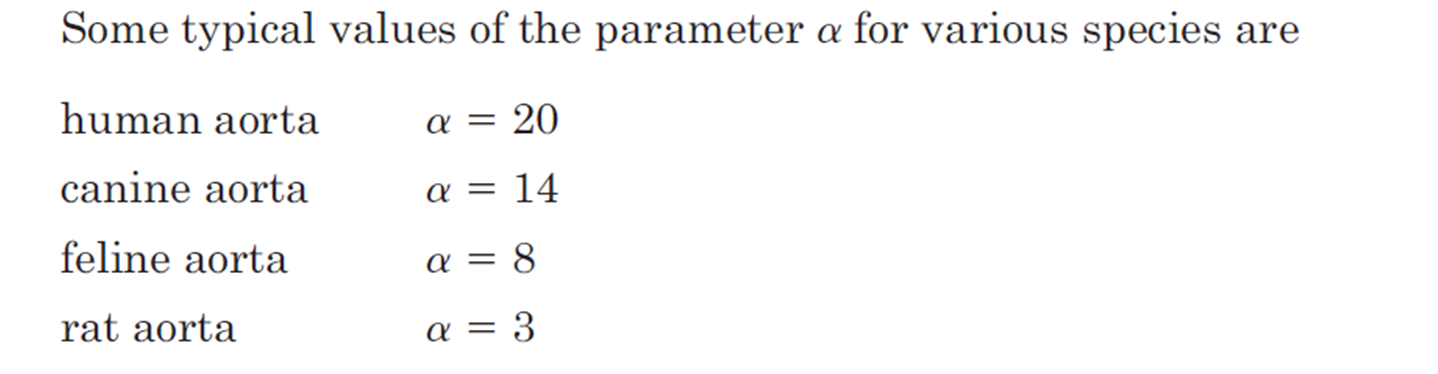
\includegraphics[scale=0.4]{Section_Files/picmanuel/42.png}
\label{fig: Figura2-35}
\end{figure}
\begin{figure}[H]
\centering
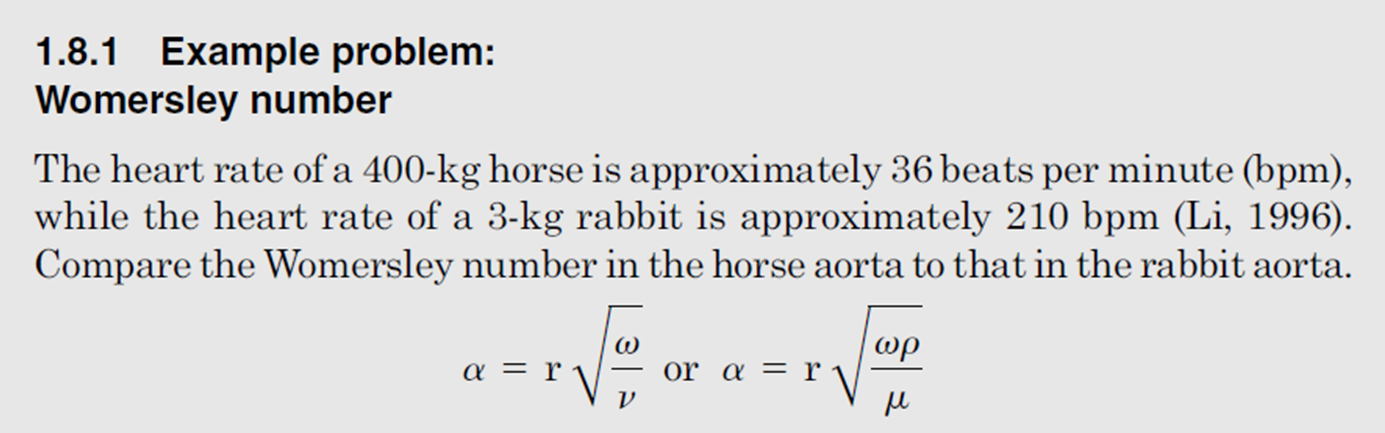
\includegraphics[scale=0.2]{Section_Files/picmanuel/43.png}
\label{fig: Figura2-36}
\end{figure}
{\tiny Tomada del libro Applied Biofluid Mechanics por Lee Wait, página 30.}
\end{frame}

\begin{frame}{Ejemplo 08 - 02/03}
\justifying
\begin{figure}[H]
\centering
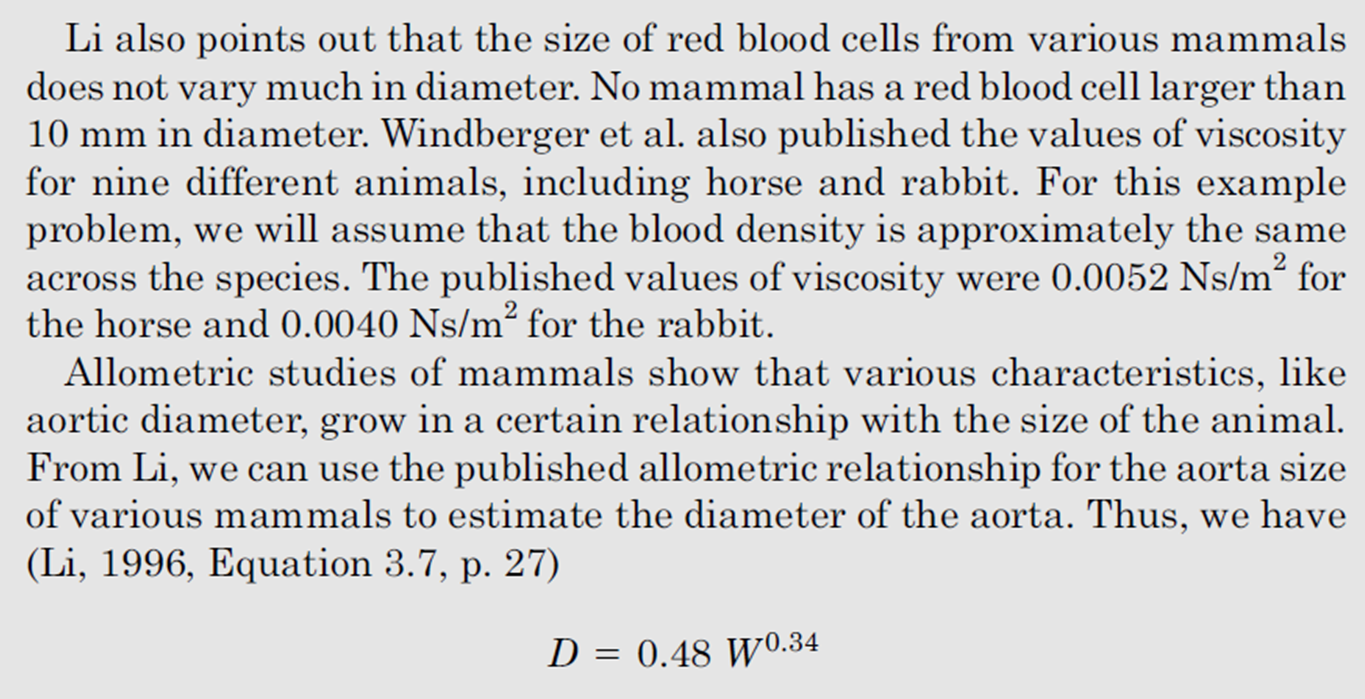
\includegraphics[scale=0.4]{Section_Files/picmanuel/44.png}
\label{fig: Figura2-37}
\end{figure}
{\tiny Tomada del libro Applied Biofluid Mechanics por Lee Wait, página 30.}
\end{frame}

\begin{frame}{Ejemplo 08 - 03/03}
\justifying
\begin{figure}[H]
\centering
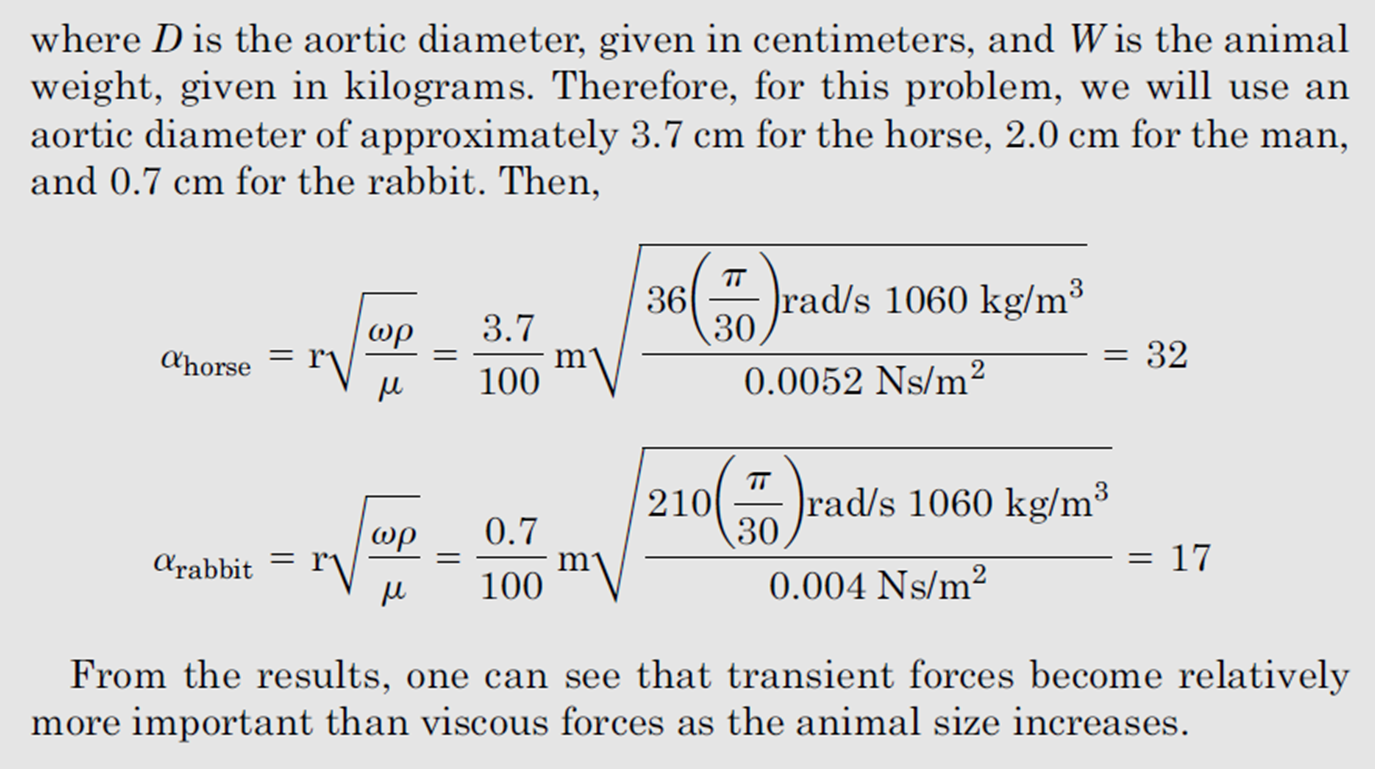
\includegraphics[scale=0.4]{Section_Files/picmanuel/45.png}
\label{fig: Figura2-38}
\end{figure}
{\tiny Tomada del libro Applied Biofluid Mechanics por Lee Wait, página 30.}
\end{frame}

\begin{frame}{Número de Strouhal (St)}
\justifying
Es un número adimensional que explica el mecanismo de un flujo oscilatorio. Esta definido como el ratio entre las fuerzas inerciales como el resultado de las condiciones de un flujo oscilatorio y las fuerzas inerciales debido a los cambios de velocidad entre dos puntos de un campo de velocidades.
\begin{figure}[H]
\centering
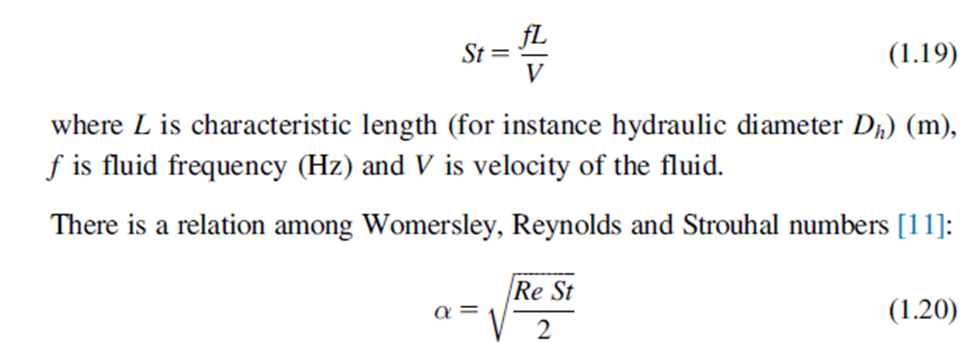
\includegraphics[scale=0.4]{Section_Files/picmanuel/46.png}
\label{fig: Figura2-39}
\end{figure}
{\tiny Tomada del libro Biofluid Mechanics Principles por Ali Ostadfar, página 18.}
\end{frame}

\begin{frame}{Número de Dean (De)}
\justifying
Esta definido como el ratio entre las fuerzas viscosas en un fluido fluyendo a través de una tubería curva y las fuerzas centrífugas.
\begin{figure}
\centering
\subfloat[a1.]{
\label{f:imagen13}
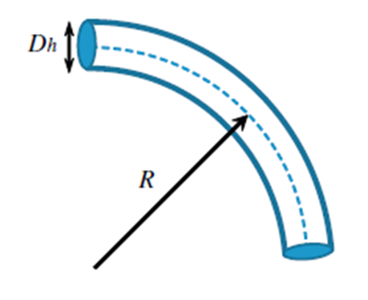
\includegraphics[height=0.30\textwidth]{Section_Files/picmanuel/47.png}}
\subfloat[b2.]{
\label{f:imagen14}
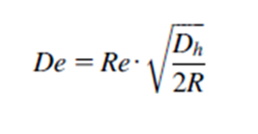
\includegraphics[height=0.30\textwidth]{Section_Files/picmanuel/48.png}}
\caption{Donde Re es el número de Reynolds, Dh es el diámetro hidráulico (m) y R es el radio de curvatura del canal.}
\label{f:numberdean}
\end{figure}
{\tiny Tomada del libro Biofluid Mechanics Principles por Ali Ostadfar, página 19.}
\end{frame}

\begin{frame}{Número de Stokes (Stk)}
\justifying
Esta definido como el ratio entre el tiempo de reacción característica de una partícula suspendida en una corriente de un fluido y el tiempo característico de un fluido. El tiempo de reacción es el tiempo que una partícula tarda en responder a los cambios de velocidad en una corriente.
\begin{figure}[H]
\centering
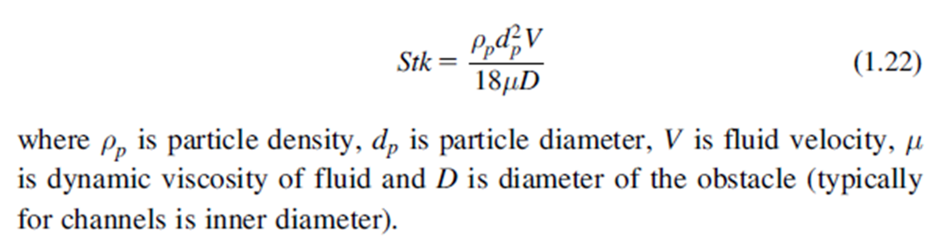
\includegraphics[scale=0.4]{Section_Files/picmanuel/50.png}
\label{fig: Figura2-40}
\end{figure}
{\tiny Tomada del libro Biofluid Mechanics Principles por Ali Ostadfar, página 19.}
\end{frame}
%*******************************************


%\subsection{4. Fluidos No-Newtoneanos}


%*******************************************


%\subsection{5. Números adimensionales aplicados a los biofluidos}
%*******************************************
